\chapter{Metody selekcji}\label{metody_selekcji}

Jednym z etapów algorytmu ewolucyjnego jest selekcja polegająca na wyborze osobników, które przedostaną się do grupy rozrodczej tworzącej potomstwo. Znanych jest kilka metod selekcji na podstawie których dokonuje się wyboru osobników z różnym prawdopodobieństwem. Metody te w większości zostały opracowane w taki sposób by dawały większe szanse przetrwania osobnikom lepiej do tego przystosowanym, a więc osobnikom o większym współczynniku funkcji przystosowania. 

Metody selekcji zostały zaimplementowane w dwojaki sposób. Pierwszym z nich jest możliwość pojawienia się danego osobnika w grupie rodzicielskiej wiecej niż jeden raz. Druga technika nakazuje różnorodność osobników w obrębie danej instancji grupy. Poniżej przestawiono idee metod selekcji podlegających rozważaniom w ramach tej pracy. Zgodnie z przyjętymi założeniami do grupy rozrodczej przedostają się 3 osobniki z populacji rodziców, co sprowadza się do faktu iż wybór należy powtórzyć trzykrotnie. Implementacje metod powstały w oparciu o \cite{maszynowe_sel}, \cite{gracjan}.

%---------------------------------------------------------------------------

\section{Losowy wybór}\label{sec:strukturaDokumentu}

Z populacji wybierany jest osobnik przechodzący do grupy rozrodczej w oparciu o  wylosowaną liczbę odpowiadającą indeksowi konkretnego osobnika. Metoda ta jest niezależna od wartości funkcji przystosowania, a więc daje równe szanse każdemu z osobników. Prawdopodobieństwo wylosowania danego osobnika, z populacji składającej się z n osobników,jest równe :
\vspace{0,4cm}
$$
P = \frac{1}{n}
$$

\par
Odpowiadająca funkcja w programie :\textbf{ RandomWitoutRestrictions()}

\begin{program}
\begin{lstlisting}[
 basicstyle=\scriptsize,]
        public List<int> RandomWitoutRestrictions()
        {
            List<int> WhichIndividuals = new List<int>();
            int number = 3;
            var rand = new System.Random();

            while (number != 0)
            {
                WhichIndividuals.Add(Kit.GiveRandomNumber(WhichIndividuals, Population.Count - 1, rand));
                number--;
            }
            return WhichIndividuals;
        }
\end{lstlisting}
\end{program}

%---------------------------------------------------------------------------

\section{Metoda rankingowa}\label{sec:kompilacja}


W metodzie selekcji rankingowej dla osobników składających się na populacje rodziców obliczana jest wartość funkcji celu, na której to podstawie tworzony jest ranking. Osobniki z najmniejszą wartością wyniku uzyskują najwyższe miejsca w rankingu \cite{selekcje}. Miejsce w rankingu jest argumentem funkcji na podstawie której obliczane jest prawdopodobieństwo wyboru danego osobnika jako rodzica. Rodzic zostanie poddany kolejnym operacjom (mutacja, krzyżowanie).\\
 Funkcja stosowana na której to podstawie tworzony jest ranking może być funkcją liniową. Wówczas osobniki zajmujące w rankingu będącym N elementowym wektorem konkretne miejsce określone rangą, gdzie N to ilość osobników w populacji otrzymują prawdopodobieństwo przejścia do grupy rodzicielskiej określone poniższą zależnością \cite{Lam92}:
$$
P = \frac{ranga}{\sum_{j=1}^{n}j}
$$

\begin{table}[h!]
\begin{center}
\begin{tabular}{|c|c|c|c|}
\hline
\textbf{Osobnik}  & \textbf{Funkcja celu} & \textbf{Ranga} & \textbf{Prawdopodobieństwo}\\
\hline
Osobnik 1 & 373 & 1 & 6,(6) \% \\
\hline
Osobnik 2 &254 & 2  & 13,(3)  \% \\
\hline
Osobnik 3 & 202 & 3 & 20  \% \\
\hline
Osobnik 4 & 136 & 4 & 26,(6)  \% \\
\hline
Osobnik 5 & 10 & 5 & 33,(3)  \% \\
\hline
\end{tabular}
\caption{Wartości parametrów na kolejnych osobników w metodzie rankingowej}
\end{center}
\end{table}

\vspace{0,4cm}

\begin{figure}[h]
		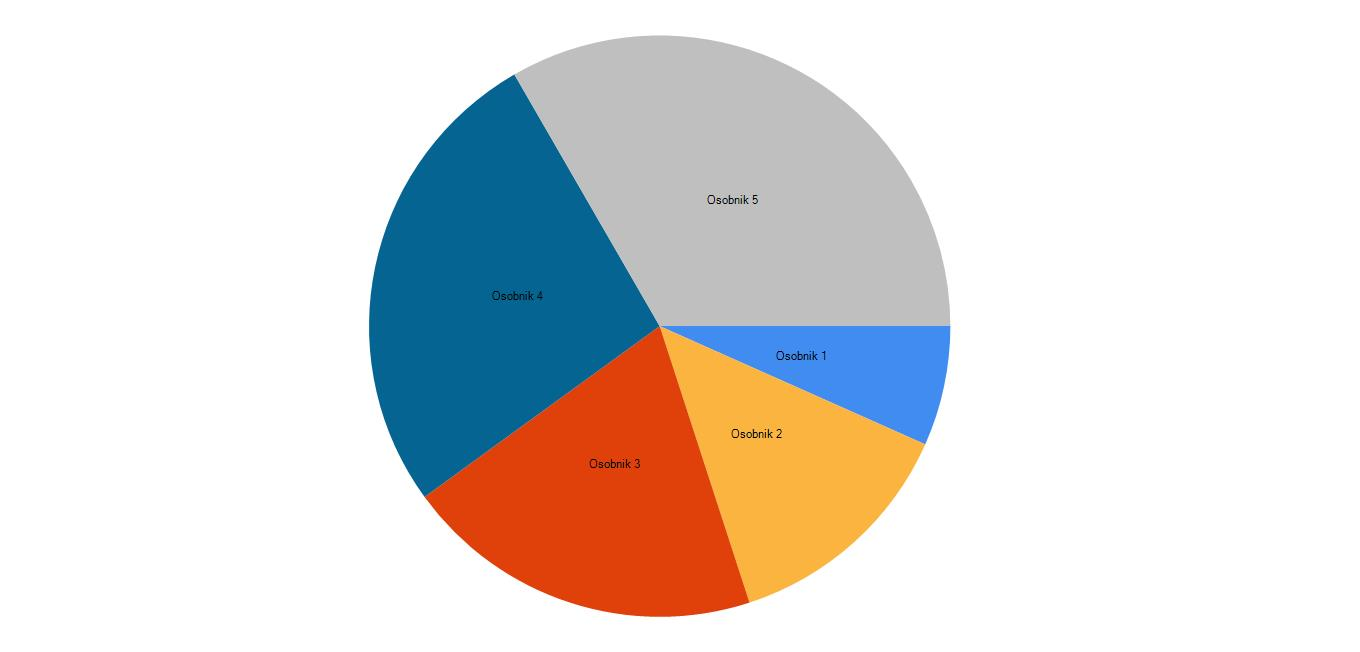
\includegraphics[scale=0.45]{../../../../Screeny/metoda_rankingowa.jpg}
		\caption{Rozkład prawdopodobieństwa w metodzie rankingowej}
		\label{ranking}			
\end{figure}
\par
Na podstawie \ref{ranking} zauważalny staje się fakt, iż rozkład prawdopodobieństwa nie jest bezpośrednio zależny od wartości funkcji celu. W metodzie tej zwiększone są więc szanse przejścia do grupy rodzicielskiej osobników z małą wartością funkcji dopasowania, które to miałyby małe szanse przejścia dalej w metodzie selekcji zależnej od wartości funkcji celu. Metoda może wydawać się niekorzystna z punktu widzenia osobników z dużą wartością funkcji dopasowania jako, że mogą otrzymać one niewiele większe prawdopodobieństwo przejścia do grupy rodzicielskiej od osobników znajdujących się range niżej pomimo iż ich wartości funkcji celu mogą różnić się znacząco.
\par
\vspace{0,4cm}
Odpowiadająca funkcja w programie : \textbf{RankingMethod()}
\begin{program}
\begin{lstlisting}[
 basicstyle=\scriptsize,]
        public List<int> RankingMethond()
        {
            List<int> WhichIndividuals = new List<int>();
            List<int> WhichIndividualsIndex = new List<int>();
            List<int> WhichIndividualBeforeSelection = new List<int>();
            List<int> ResultsOfObjectiveFunction = inputdata.ObjectiveFunctionVector(Population);

            var rand = new System.Random();
            int size_tmp = size;
            int number = 3;

            while (size_tmp != 0)
            {
                var index = ResultsOfObjectiveFunction.IndexOf(ResultsOfObjectiveFunction.Min());
                ResultsOfObjectiveFunction[index] = Int32.MaxValue;

                int numberOfIter = size_tmp;
                while (numberOfIter != 0)
                {
                    WhichIndividualBeforeSelection.Add(index);
                    numberOfIter--;
                }
                size_tmp--;
            }

            while (number != 0)
            {
                var tmp = Kit.GiveRandomNumber(WhichIndividualsIndex, WhichIndividualBeforeSelection.Count - 1, rand);
                for (int i = 0; i < WhichIndividualBeforeSelection.Count; i++) // to w celu uniknięcia powtórzeń w wektorach
                {
                    if (WhichIndividualBeforeSelection[i] == WhichIndividualBeforeSelection[tmp])
                        WhichIndividualsIndex.Add(i);
                }

                WhichIndividuals.Add(WhichIndividualBeforeSelection[tmp]);
                number--;
            }
            return WhichIndividuals;
        }
\end{lstlisting}
\end{program}

%---------------------------------------------------------------------------

\section{Metoda ruletki}\label{sec:narzedzia}


W metodzie ruletki każdemu chromosomowi zostaje przypisany wycinek koła \cite{selekcje}. Im silniejszy osobnik tym większy wycinek koła dostaje, gdyż zależność wartości funkcji przystosowania i prawdopodobieństwo wylosowania osobnika jest wprost proporcjonalna. Każdy osobnik tworzący populacje poddawany jest ocenie funkcji celu. Maksymalna wartość funkcji przystosowania oznacza najmniejszą wartość funkcji celu. Uzyskana wartość funkcji przystosowania w stosunku do sum wartości tej funkcji wszystkich osobników populacji wyznacza prawdopodobieństwo wylosowania danego osobnika na rodzica. Prawdopodobieństwo wylosowania danego osobnika dane jest następującą zależnością:
$$
P_i = \frac{f(i)}{\sum_{j=1}^{n}f(j)}
$$
Gdzie f(x) - funkcja przystosowania\\
\par
Funkcją przystosowania w rozważanym poniżej przypadku jest funkcja przyporządkowującą największej wartości funkcji celu wartość najmniejszą, a wartości najmniejszej wartość największą.

\begin{table}[h!]
\begin{center}
\begin{tabular}{|c|c|c|c|}
\hline
\textbf{Osobnik}  & \textbf{Funkcja celu} & \textbf{Funkcja dopasowania} & \textbf{Prawdopodobieństwo}\\
\hline
Osobnik 1 & 373 & 10 & 1,02  \% \\
\hline
Osobnik 2 &254 & 136  & 13,95  \% \\
\hline
Osobnik 3 & 202 & 202 & 20,72  \% \\
\hline
Osobnik 4 & 136 & 254 & 26,05  \% \\
\hline
Osobnik 5 & 10 & 373 & 38,25  \% \\
\hline
\end{tabular}
\caption{Wartości parametrów na kolejnych osobników w metodzie ruletki}
\end{center}
\end{table}

\vspace{0,4cm}

\begin{figure}[h]
		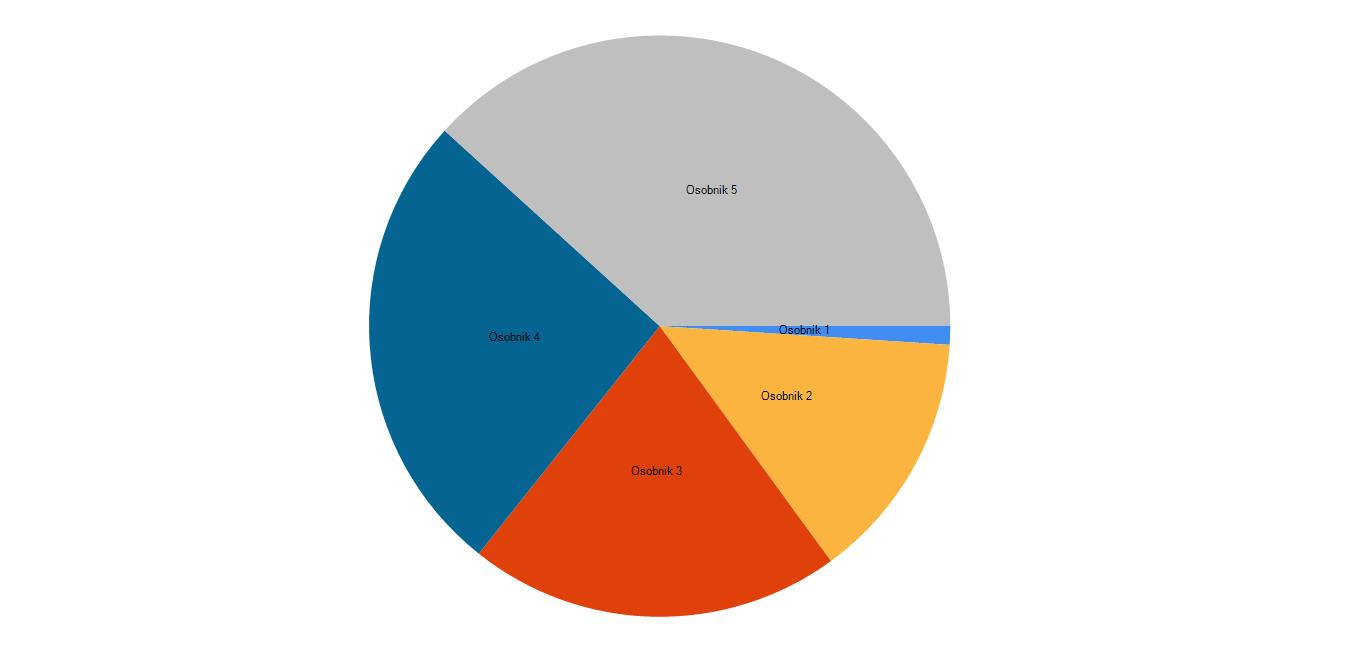
\includegraphics[scale=0.45]{../../../../Screeny/metoda_ruletki.jpg}
		\caption{Rozkład prawdopodobieństwa w metodzie ruletki}
		\label{ruletka}			
\end{figure}
\par
W metodzie ruletki wkład każdego osobnika w rozkład prawdopodobieństwa jest wprost proporcjonalny do wartości jego funkcji dopasowania. Wady tej metody stają się widoczne, w sytuacji gdy dany osobnik zajmuje większość powierzchni koła, gdyż osobniki o małej wartości funkcji dopasowania są przedwcześnie eliminowane, a więc nie mają wielkiej szansy by zostać wylosowane. Prowadzi to do braku różnorodności w kolejnych grupach rozrodczych, co utrudnia dojście do lepszego wyniku. Z problemem tym dobrze sobie radzi wspomniana wyżej metoda rankingowa gzdei eliminowana jest możliwość dużej przewagi jednego z nich nad resztą.\\
\par
Odpowiadająca funkcja w programie : \textbf{RouletteMethod()}

\begin{program}
\begin{lstlisting}[
 basicstyle=\scriptsize,]
        public List<int> RouletteMethond()
        {
            List<int> WhichIndividuals = new List<int>();
            List<int> ResultsOfObjectiveFunction = inputdata.ObjectiveFunctionVector(Population);
            List<Tuple<int, int>> tuple = new List<Tuple<int, int>>();
            int range_begin = 0;
            int range_end = 0;
            var rand = new System.Random();
            int number = 3;

            foreach (var elem in ResultsOfObjectiveFunction)
            {
                range_end += elem;
                tuple.Add(new Tuple<int, int>(range_begin, range_end));
                range_begin = elem + 1;
            }

            while (number != 0)
            {
                var tmp = Kit.GiveRandomNumber(WhichIndividuals, ResultsOfObjectiveFunction.Sum(), rand);
                for (int i = 0; i < tuple.Count; i++)
                {
                    if (tuple[i].Item2 > tmp)
                    {
                        WhichIndividuals.Add(i);
                        number--;
                        break;
                    }
                }
            }
            return WhichIndividuals;
        }
\end{lstlisting}
\end{program}

%---------------------------------------------------------------------------

\section{Metoda turniejowa}\label{sec:narzedzia}


Metoda selekcji turniejowej polega na rozgrywaniu turnieju pomiędzy osobnikami tworzącymi populacje. W wyniku jednorazowej rozgrywki wygrywa osobnik o większej wartości funkcji przystosowania, przechodząc tym samym do kolejnej rundy. W każdym turnieju zwycięża jeden osobnik, którego to genotyp jest wykorzystywany przy kolejnych operacjach genetycznych. Populacja dzielona jest na dwuosobnikowe podgrupy w których to dokonywane są rozgrywki. W przypadku nieparzystego rozmiaru populacji, osobnik ostatni przechodzi do kolejnej rundy bezkonkurencyjnie. \\
\par
Metoda turniejowa nie wymaga znajomości optymalizowanej funkcji, konieczny jest jedynie informacja o relacji zachodzącej pomiędzy dwoma kolejnymi osobnikami. 
\par
Odpowiadająca funkcja w programie : \textbf{TournamentMethod()}

\begin{program}
\begin{lstlisting}[
 basicstyle=\scriptsize,]
 public List<int> TournamentMethond()
        {
            List<int> WhichIndividuals = new List<int>();
            List<int> ResultsOfObjectiveFunction = inputdata.ObjectiveFunctionVector(Population);
            List<int> ResultsOfObjectiveFunction_const = new List<int>();
            ResultsOfObjectiveFunction_const.AddRange(ResultsOfObjectiveFunction);
            List<int> TournamentTable = new List<int>();
            int number = 3;

            while (number != 0)
            {
                int sizeOfTournament_const = ResultsOfObjectiveFunction.Count;
                while (sizeOfTournament_const > 1)
                {
                    for (int i = 0; i < sizeOfTournament_const; i++)
                    {
                        TournamentTable.Add(Math.Min(ResultsOfObjectiveFunction[i], ResultsOfObjectiveFunction[i + 1]));
                        i++;

                        if ((sizeOfTournament_const \% 2) == 1 \&\& i == sizeOfTournament_const - 2)
                        {
                            TournamentTable.Add(ResultsOfObjectiveFunction.Last());
                            i++;
                        }
                    }

                    if (TournamentTable.Count == 1)
                        break;
                    sizeOfTournament_const = TournamentTable.Count;
                    ResultsOfObjectiveFunction.RemoveAll(elem => ResultsOfObjectiveFunction.Contains(elem));
                    ResultsOfObjectiveFunction.AddRange(TournamentTable);
                    TournamentTable.RemoveAll(elem => TournamentTable.Contains(elem));
                }

                var index = ResultsOfObjectiveFunction_const.FindIndex(value => value == TournamentTable[0]);
                WhichIndividuals.Add(index);
                ResultsOfObjectiveFunction_const[index] = Int32.MaxValue;
                ResultsOfObjectiveFunction.RemoveAll(elem => ResultsOfObjectiveFunction.Contains(elem));
                ResultsOfObjectiveFunction.AddRange(ResultsOfObjectiveFunction_const);
                TournamentTable.RemoveAt(0);
                number--;
            }
            return WhichIndividuals;
        }
\end{lstlisting}
\end{program}

%---------------------------------------------------------------------------

\section{Metoda elitarna}\label{sec:przygotowanieDokumentu}

W metodzie tej nacisk położony jest na to, aby do grupy rozrodczej przedostały się z prawdopodobieństwem równym p=100\% osobniki najlepiej przystosowane. W poprzednich metodach(ruletki, turniejowa, rankingowa) prawdopodobieństwo przejścia do grupy rozrodczej dla osobników z większym wskaźnikiem funkcji przystosowania jest jedynie większe niż dla pozostałych osobników. Nie ma jednak gwarancji przedostania się dalej osobników najlepiej przystosowanych. W strategii elitarnej do grupy na której zostanie dokonana operacja mutacji a następnie krzyżowania przedostaje się n osobników z populacji odznaczających się najwyższym wskaźnikiem funkcji przystosowania \cite{GPS}.\\
\par
Zastosowanie elitaryzmu jako metody selekcji daje pewność iż do grupy rodzicielskiej przedostaną się najlepiej do tego przystosowane osobniki. Dzięki temu unika sie sytuacji w której stosunkowo mocny osobnik w wyniku operacji genetycznych zostanie osłabiony a co za tym idzie, nie przechodzi on do grupy rodzicielskiej.\\
\par
Odpowiadająca funkcja w programie : \textbf{ElitistMethod()}

\begin{program}
\begin{lstlisting}[
 basicstyle=\scriptsize,]
        public List<int> ElitistMethond()
        {
            List<int> WhichIndividuals = new List<int>();
            List<int> ResultsOfObjectiveFunction = inputdata.ObjectiveFunctionVector(Population);
            int number = 3;

            while (number != 0)
            {
                int index = ResultsOfObjectiveFunction.FindIndex(min => min == ResultsOfObjectiveFunction.Min());
                WhichIndividuals.Add(index);
                ResultsOfObjectiveFunction[index] = Int32.MaxValue;
                number--;
            }

            return WhichIndividuals;
        }
\end{lstlisting}
\end{program}

